% =====================================================================
% ECC 2027 draft (ieeeconf). Object: the limit cycle of fixed-step SPIN.
% Deterministic theory: closed orbits (combinatorial, any index),
% localization and the small-step limit (topological, any index), and the
% published count as the limit of a continuous count. Robustness: the
% orbits sit on the event "overshoot = delta", a damping condition on the
% step response of S.
%
% Every number is produced by docs/ECC27_limit_cycle/scripts/lc_results.py
% from the current code (lc_results.json); nothing is quoted from earlier
% drafts. Setting: lc_setup.py.
% =====================================================================
\documentclass[letterpaper, 10 pt, conference]{ieeeconf}
\IEEEoverridecommandlockouts
\overrideIEEEmargins

\usepackage{amsmath,amssymb}
\usepackage{graphicx}
\usepackage{booktabs}
\usepackage{url}

\newtheorem{lemma}{Lemma}
\newtheorem{proposition}{Proposition}
\newtheorem{theorem}{Theorem}
\newtheorem{corollary}{Corollary}
\newtheorem{assumption}{Assumption}
\newtheorem{remark}{Remark}
\renewenvironment{proof}{\noindent\textit{Proof:}\ }{\hfill$\square$\par\smallskip}

\newcommand{\Nbar}{\bar{N}}
\newcommand{\spin}{SPIN}

\title{\LARGE\bf Limit Cycles of Model-Free PID Tuning\\ by Step-Response Inspection}

\author{Pavel Otta$^{1}$, Daniel Pachner$^{1}$, Ji\v{r}\'{\i} Dost\'al$^{1}$
and Vladim\'{\i}r Havlena$^{2}$%
\thanks{$^{1}$University Centre for Energy Efficient Buildings (UCEEB),
Czech Technical University in Prague, Bu\v{s}t\v{e}hrad, Czech Republic.
Corresponding author: {\tt pavel.otta@cvut.cz}}%
\thanks{$^{2}$Department of Control Engineering, Faculty of Electrical
Engineering, Czech Technical University in Prague, Czech Republic.}%
}

\begin{document}
\maketitle
\thispagestyle{empty}
\pagestyle{empty}

\begin{abstract}
\spin{} tunes a PID controller from closed-loop step responses: it counts
how often three phase portraits of the error turn around the origin and
moves the gains by a fixed table of four moves. In every run we made, the
iteration ends in a periodic orbit. We characterize such orbits in the
deterministic case. Every closed orbit that stays below the upper gain
bound, whatever turn index drives the rule, applies the four moves in the
proportions $1\!:\!4\!:\!2\!:\!1$, has a period of $8 n_e$ for an integer
multiplicity $n_e$, and stays within $n_e (2, 1, \tfrac12)$ steps of its
centre in $(\log K_i, \log K_p, \log K_d)$. Its bounding box meets the
switching boundaries, so as the step shrinks the orbits accumulate where the
boundaries meet. For the published turn count this set is not a point. The
count is the limit of a continuous count that makes the rule's move on
$98.5$--$99.5\,\%$ of the states the rule visits, and through it the
destination becomes visible: all $108$ terminal orbits on a four-plant
battery straddle the event at which the overshoot of the step response
equals the settling band $\delta = 2\,\%$, and every quiet step has a smaller
overshoot. This is a damping condition on the step response of the
sensitivity function $S$. The orbits therefore differ in the gains but
hardly in robustness: the largest sensitivity peak on an orbit lies within
$1.54$--$2.10$ when the derivative acts on the error, and reaches $2.95$ when it
acts on the measurement and the record is no longer the step response of $S$.
A plant-free step-size rule and a drift meter follow from the orbit structure.
\end{abstract}

% =====================================================================
\section{Introduction}

Most PID tuning methods first fit a model and then compute the gains
\cite{ZN1942,AstromHagglund2004}. \spin{} \cite{Paper1} tunes from what the
closed-loop step response looks like instead. It draws three phase portraits
of the control error, counts how often each turns around the origin, compares
the three \emph{turn counts} $N_k$ with fixed thresholds $\Nbar_k$, and applies
one of four moves to the gains. No model is identified. Iterative feedback
tuning \cite{Hjalmarsson1998} and extremum seeking \cite{Killingsworth2006}
estimate gradients of a cost; the triangular rule uses only three signs.
Its natural end state is therefore not a stationary point but a periodic
orbit of a switched system, and this paper is about that orbit.

We ask where the orbit is, what shape it has, what happens to it as the step
shrinks, and why it ends at a robust controller. The answers come in three
layers. The first is combinatorial and holds for any turn index: the move
counts, the period and the excursion of every closed orbit
(Section~\ref{sec:orbits}). The second is topological and also holds for any
index: the orbit's box meets the switching boundaries, so small-step orbits
accumulate on their intersection (Section~\ref{sec:limit}). The third
concerns the published count, a winding number over a window that ends when
the error settles, which jumps when that window jumps. We construct a
continuous count of which it is the limit, find that the orbits sit on the
event at which the overshoot equals the settling band $\delta$, and read that
event as
a damping condition on the sensitivity function
(Sections~\ref{sec:count}--\ref{sec:robust}). This explains why the
destination is not unique and why it is robust anyway.
Section~\ref{sec:step} turns the orbit structure into a step-size rule and a
stopping test.

% =====================================================================
\section{The Rule as a Switched System}
\label{sec:rule}

\emph{Loop and record.} A discrete-time loop with sampling period $T_s$
closes a parallel PID controller $K_p + K_i/s + K_d s/(1 + (K_d/\nu) s)$,
$\nu = 10$, around the plant, and a unit setpoint step is applied at
$t = 0$. The record is the error $e_n = r - y_n$, $n = 0, \dots, n_{\max}$.

\begin{assumption}\label{ass:loop}
The loop is linear and noise-free, and the derivative acts on the error.
\end{assumption}

Under Assumption~\ref{ass:loop} the increments $e_n - e_{n-1}$ ($e_{-1} = 0$)
are the impulse response of the sensitivity function $S$, so the record is
the step response of $S$ \cite{Certified}. We return to this in
Section~\ref{sec:robust}.

\emph{Turn counts.} From the record, \spin{} draws three portraits:
$\Gamma_0 = (e, E)$ with $E$ the running sum of $e$, $\Gamma_1 = (\Delta e, e)$
and $\Gamma_2 = (\Delta^2 e, \Delta e)$. They are read over a window
$[k_1, k_\delta]$. The start $k_1$ is the first sample at which the output
has risen past $10\,\%$ of the step, plus a fixed padding. The end $k_\delta$
is one sample past the last sample with $|e_n| > \delta \max_m |e_m|$,
$\delta = 0.02$, clipped to $[k_1, k_2]$, where $k_2$ is the end of the record
less a padding. Each axis is normalized by its peak over the window, the
integral axis of $\Gamma_0$ is taken relative to its value at $k_\delta$, and the
turn count $N_k$ is the winding number of $\Gamma_k$ around the origin, up to
the last segment that touches the disc of radius $\varepsilon = 0.1$. The
thresholds are $\Nbar = (0.5, 0.75, 1.0)$.

\emph{Moves.} We write $\theta = (\log K_i, \log K_p, \log K_d)$, in band order.
If the stability screen of \cite{Paper1} finds the record growing, all gains
are backed off by $b = (1, 2, 3) \log 2$. Otherwise the lowest band with
$N_k > \Nbar_k$ is cut and the bands below it are raised; if no band is
violated, all are raised. With $h = \log\gamma$, $\gamma = 1/(1-\beta)$, the four
moves are translations by $h$ times
\begin{equation}
\begin{aligned}
g &= (1, 1, 1), & d_0 &= (-1, 0, 0),\\
d_1 &= (1, -1, 0), & d_2 &= (1, 1, -1).
\end{aligned}
\label{eq:moves}
\end{equation}
A $g$-step (``grow'') is \emph{quiet}: it is taken only where no band is
violated. The gains live in the box $\Theta = [\ell, u]^3$,
$\ell = \log 10^{-3}$, $u = \log 10$; raises are clipped at $u$ and cuts at
$\ell$. We use $\beta = 0.1$ unless stated.

\emph{Two corrections to \cite{Paper1}.} (i)~A cut is \emph{blocked} if its
gain is already at $\ell$. A blocked cut now passes to the nearest lower band
whose gain can still be cut, with the raises below that band; if there is
none, the gains are held. Previously the raises were applied although the
cut was not, which applied the vector $(1, 1, 0)$, outside the table
\eqref{eq:moves}. (ii)~The winding number is computed as the sum of the
signed angles of the portrait's segments. The published implementation
corrected the endpoint angle by crossings of the negative real axis but
missed crossings by a segment with one end at $x \ge 0$, and on the last
segment; it miscounted by one or two full turns on $41$ of the $8792$ states
visited in Section~\ref{sec:count}. Both corrections are in the reference
code.

\emph{Experiments.} The battery is that of \cite{Paper1}: P1
$e^{-s}/((10s+1)(s+1)^3)$, P2 $1.25e^{-8s}/(5s+1)^4$, P3
$e^{-10s}/((2s+1)(s+1)^3)$, P4 $e^{-4s}/(8s+1)^6$. Each record has $500$
samples over ten times the sum of the plant's time constants and dead time.
For each plant we start from the AMIGO gains \cite{AstromHagglund2004} and
from the $26$ gain vectors obtained by multiplying each AMIGO gain by $8$,
$1$ or $1/8$, and run the deterministic iteration until it revisits a state.
The states from the first visit on form the terminal orbit.

% =====================================================================
\section{Closed Orbits}
\label{sec:orbits}

\begin{lemma}\label{lem:table}
Let $\log 2/h$ be irrational. On a closed orbit of period $T \ge 2$ that does
not reach the ceiling $u$ and on which $K_i$ stays above $\ell$, every step
is a full table move $\theta^{t+1} = \theta^t + h v^t$,
$v^t \in \{g, d_0, d_1, d_2\}$.
\end{lemma}

\begin{proof}
A step is a table move, possibly with a cut clipped at $\ell$; a raise
clipped at $u$; a screen backoff, possibly clipped at $\ell$; or a hold. A
hold is a fixed point ($T = 1$), and clipped raises are excluded. The
coordinate $\log K_i$ is never clipped, so its steps are $0$, $\pm h$ or
$-\log 2$; closing the orbit gives $m h = n \log 2$ with $n$ the number of
screen events, hence $n = 0$. In $\log K_p$ and $\log K_d$ the remaining
steps are $0$, $\pm h$ and cuts clipped to $\ell$. If a coordinate takes the
value $\ell$ on the orbit, then following the orbit from there it takes only
values in $\ell + h\mathbb{Z}$, since $\pm h$ preserves this set and a clipped
cut would start in $(\ell, \ell + h)$; so no cut is clipped. If it never
takes the value $\ell$, no cut is clipped either. By correction~(i), a
passed-on cut is a table move of a lower band.
\end{proof}

For $\beta = 0.1$, $\log 2/\log(10/9)$ is irrational: $2^q = (10/9)^p$ would
give $2^{q} 3^{2p} = 2^p 5^p$.

\begin{proposition}[Balance]\label{prop:balance}
The only convex combination of the moves \eqref{eq:moves} that vanishes is
$\tfrac18 g + \tfrac12 d_0 + \tfrac14 d_1 + \tfrac18 d_2 = 0$.
\end{proposition}

\begin{proof}
With weights $w$, the $\log K_d$ coordinate gives $w_g = w_2$, then
$\log K_p$ gives $w_1 = 2 w_g$, $\log K_i$ gives $w_0 = 4 w_g$, and
$\sum w = 1$ gives $w_g = \tfrac18$.
\end{proof}

\begin{theorem}[Closed orbits]\label{thm:orbit}
Under the hypotheses of Lemma~\ref{lem:table}, the orbit applies the moves
$(g, d_0, d_1, d_2)$ exactly $n_e (1, 4, 2, 1)$ times for an integer
$n_e \ge 1$, its \emph{multiplicity}; so $T = 8 n_e$ and every move occurs.
Each coordinate stays within $n_e (2, 1, \tfrac12)\, h$ of the midpoint of
its range on the orbit; we call the vector of these midpoints the orbit's
\emph{centre}.
\end{theorem}

\begin{proof}
By Lemma~\ref{lem:table} the counts $n_v$ satisfy $\sum_v n_v v = 0$; the
computation of Proposition~\ref{prop:balance} over the integers gives
$n = n_e(1,4,2,1)$, and $T \ge 2$ forces $n_e \ge 1$. A closed walk with
$m$ up-steps and $m$ down-steps of size $h$ has range at most $m h$; per
period, $\log K_i$, $\log K_p$ and $\log K_d$ are raised $4n_e$, $2n_e$ and
$n_e$ times.
\end{proof}

On the battery, the six P4 orbits that reach the $K_d$ ceiling are excluded
by the hypotheses; five of them have period four. All other $102$ orbits have
the predicted counts and lie within the bound; $93$ have $n_e = 1$, the others
$n_e \in \{2, 3, 4, 5, 9, 24\}$. Three of P1's, thirteen of P2's and fifteen
of P4's orbits have $K_d$ on the floor, where passed-on cuts keep the table
intact. From the AMIGO start every plant closes an orbit of period eight after
$9$ to $19$ experiments.

The table \eqref{eq:moves} is not an arbitrary choice.

\begin{proposition}[The table is forced]\label{prop:forced}
Among tables for $n$ bands with entries in $\{-1, 0, 1\}$, $g = (1, \dots, 1)$
and $d_k[k] = -1$, the staircase table ($d_k[j] = 1$ for $j < k$, $0$ for
$j > k$), which is \eqref{eq:moves} for $n = 3$, is the only one whose balance
weights equal the frequencies with which the priority logic selects the
moves when the $n$ signs $N_k \gtrless \Nbar_k$ are equally likely.
\end{proposition}

\begin{proof}
The logic selects $g$ on $1$ of the $2^n$ sign patterns and $d_k$ on
$2^{n-k-1}$. Matching requires $g + \sum_k 2^{n-k-1} d_k = 0$; coordinate $j$
reads $\sum_k 2^{n-k-1} d_k[j] = -1$, a signed-binary representation of $-1$.
The $n$ such representations have a single $-1$ digit at a position $m$,
with $d_k[j] = +1$ for $k > m$ and $0$ for $k < m$. The hypothesis
$d_j[j] = -1$ forces $m = j$, which is the staircase.
\end{proof}

A consequence for noise: if noise makes the comparisons independent fair
coins, the moves occur at the balance weights and the expected displacement
is zero. The balance point does not drift; only the spread grows.

% =====================================================================
\section{Localization and the Small-Step Limit}
\label{sec:limit}

Let $\Sigma_k$ be the boundary of the set
$\{\theta \in \Theta : N_k(\theta) > \Nbar_k\}$: the switching boundary of
band $k$. No continuity of $N$ is assumed.

\begin{proposition}[Localization]\label{prop:local}
Let a closed orbit satisfy Theorem~\ref{thm:orbit}, and let $B$ be its
bounding box. Then $B$ meets $\Sigma_2$. If no cut on the orbit is passed
on, $B$ meets $\Sigma_0$, $\Sigma_1$ and $\Sigma_2$.
\end{proposition}

\begin{proof}
The orbit contains a quiet step, taken where $N \le \Nbar$, and a $d_2$-step,
taken only where $N_2 > \Nbar_2$. Without passed-on cuts, a $d_k$-step is
taken only where $N_k > \Nbar_k$. The box is connected and contains points of
$\{N_k > \Nbar_k\}$ and of its complement, so it meets the boundary.
\end{proof}

\begin{corollary}[Small-step limit]\label{cor:limit}
Let $\beta_j \to 0$, and let the orbits $O_j$ satisfy
Proposition~\ref{prop:local} without passed-on cuts, with
$n_e^{(j)} h_j \to 0$. Every accumulation point of $O_j$ lies in
$\mathcal{T} = \Sigma_0 \cap \Sigma_1 \cap \Sigma_2$.
\end{corollary}

\begin{proof}
The diameter of $B_j$ is at most $\sqrt{21}\, n_e^{(j)} h_j \to 0$ by
Theorem~\ref{thm:orbit}; each $B_j$ meets each closed set $\Sigma_k$.
\end{proof}

\begin{remark}[Transversal case]\label{rem:transversal}
If $N$ is $C^1$ near a point $\theta^*$ with $N(\theta^*) = \Nbar$ and a
nonsingular Jacobian $J^*$, then $\mathcal{T}$ is locally $\{\theta^*\}$. A box
$B$ near $\theta^*$ that meets the three level sets satisfies
$|N_k - \Nbar_k| \le \lVert \nabla N_k \rVert \operatorname{diam} B$ at its
centre by the mean-value theorem, and the inverse function theorem turns this
into a distance $O(\lVert (J^*)^{-1} \rVert \lVert J^* \rVert
\operatorname{diam} B)$ from $\theta^*$. For orbits of bounded multiplicity
without passed-on cuts this is a rate $O(h)$.
\end{remark}

The existence and attraction of a terminal orbit remain open; what the
results above fix is where any closed orbit can be, and where small-step
orbits must end up. On the battery, from the AMIGO start, halving $\beta$ from
$0.1$ to $0.00625$ moves the orbit centre by $0.39$, $0.031$, $0.015$ and
$0.007$ on P1 and by $0.18$, $0.041$, $0.020$ and $0.002$ on P2 (in
$\log$-gain): the centres converge. On P3 the centre jumps once ($0.25$ at
$\beta = 0.025$) and then moves by less than $0.01$; on P4 the orbits reach the
$K_d$ ceiling for $\beta \le 0.05$. What $\mathcal{T}$ looks like depends on
the count.

% =====================================================================
\section{The Published Count as a Limit}
\label{sec:count}

The published count is a composition of discrete steps: the window start
$k_1$, the window end $k_\delta$, the peak normalization over the window,
the reference value of $\Gamma_0$'s integral axis at $k_\delta$, and the cut
at the last disc contact. Each makes $N$ jump. We replace each by a smooth
version. Let $\psi$ be the logistic function and
$A_n = \max_{m \ge n} |e_m| / \max_m |e_m|$ the \emph{future envelope} of the
error. Sample $n$ is before the window end with weight
$P_n = \psi(p \log(A_{n-1}/\delta))$, the smooth version of $n \le k_\delta$,
and after the window start with weight
$Q_n = \psi(p_s (0.9 - \min_{m \le n - \kappa} e_m))$, $\kappa$ the padding.
Each portrait axis is normalized by $\max_n Q_n P_n |a_n|$, and $\Gamma_0$'s
reference value is $\sum_n (P_n - P_{n+1}) E_n$. Segment $n$ of a portrait,
from $(a_n, b_n)$ to $(a_{n+1}, b_{n+1})$, turns by
$\varphi_n = \operatorname{atan2}(a_n b_{n+1} - b_n a_{n+1},\,
a_n a_{n+1} + b_n b_{n+1})$ and counts with the weight
$\omega_n = Q_n P_{n+1} V_n\, \rho_n^2/(\rho_n^2 + r_0^2)$. Here $\rho_n$ is
the segment's distance from the origin, and $V_n$ is the smooth version of
``a later segment touches the disc, or no segment does'', built from
$\psi(p \log(\varepsilon/\rho_m))$. The continuous count of band $k$ is
\begin{equation}
N_{k,p} = \frac{1}{2\pi} \sum_n \omega_n \varphi_n
\label{eq:smooth}
\end{equation}
over the portrait $\Gamma_k$. We use $p = 32$, $p_s = 200$ and
$r_0 = \varepsilon/100$.

\begin{proposition}[Continuity and limit]\label{prop:smooth}
For finite $p$, $p_s$ and $r_0 > 0$, $N_p$ is a continuous function of the
record wherever the record and the portrait axes are not identically zero;
under Assumption~\ref{ass:loop} it is therefore continuous in $\theta$. As
$p, p_s \to \infty$ and $r_0 \to 0$, $N_p$ tends to the published count at
every record without ties ($|e_n| = \delta \max|e|$, the output exactly at the
$10\,\%$ level, a segment at distance exactly $\varepsilon$ or through the
origin), except when the last disc contact is on the second segment, where
the published count is set to zero.
\end{proposition}

\begin{proof}
Envelopes, extrema, logistics and products are continuous. The segment angle
is discontinuous only where the segment passes through the origin, where
$\rho_n = 0$ and its weight vanishes, so the product is continuous. A finite
linear recursion makes the record continuous in the gains. As the
sharpnesses grow, each logistic tends to the indicator it smooths, off the
ties.
\end{proof}

Table~\ref{tab:fidelity} measures the limit and the agreement on the states
visited in the first $120$ iterations from each of the $27$ starts. The hard
limit coincides with the published count on $8791$ of $8792$ states, the
exception being the second-segment case. At $p = 32$ the continuous count makes
the rule's move on $98.5$--$99.5\,\%$ of the states, and driving the rule with
it reaches the same terminal orbit from $67$--$100\,\%$ of the starts; from the
others it reaches another orbit of the kind described next.

\begin{table}[t]
\centering\small
\caption{The continuous count against the published one, on the states
visited in the first $120$ iterations from each of $27$ starts per plant.}
\label{tab:fidelity}
\setlength{\tabcolsep}{4pt}
\begin{tabular}{lrcccc}
\toprule
 & states & hard limit & \multicolumn{2}{c}{same move} & same orbit \\
 & & exact & $p=8$ & $p=32$ & $p=32$ \\
\midrule
P1 & 1926 & 1926 & $95.6\,\%$ & $98.8\,\%$ & $20/27$ \\
P2 & 2332 & 2332 & $96.2\,\%$ & $98.9\,\%$ & $21/27$ \\
P3 & 2216 & 2215 & $96.4\,\%$ & $98.5\,\%$ & $18/27$ \\
P4 & 2318 & 2318 & $97.6\,\%$ & $99.5\,\%$ & $27/27$ \\
\bottomrule
\end{tabular}
\end{table}

\emph{Where the orbits sit.} Let the overshoot be the largest excursion of the
output above the setpoint, relative to $\max|e|$. While it is below $\delta$,
the window ends before the overshoot lobe and the portraits do not contain
it; once it exceeds $\delta$, the window end $k_\delta$ jumps past the lobe, and
since the window is shared by the three portraits, all three counts jump
together (Fig.~\ref{fig:index}). This \emph{overshoot event} is where every
orbit sits. All $108$ terminal orbits straddle it: each has points with
overshoot below and above $\delta$. Every quiet step on every orbit has an
overshoot below $\delta$ (at most $1.96\,\%$), while $68$--$75\,\%$ of the
corrective steps, by plant, have one above it (median $3.5$--$7.6\,\%$). Where
the jump carries a count across its threshold, as for $N_0$ in
Fig.~\ref{fig:index}, the switching boundary of that band is a piece of the
event surface.

\begin{figure}[t]
\centering
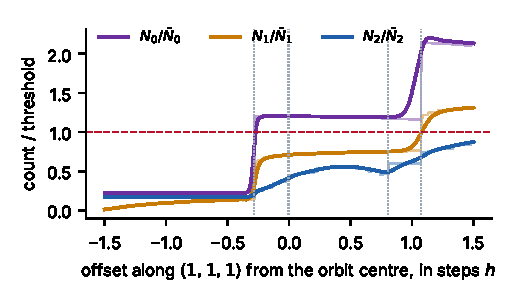
\includegraphics[width=\linewidth]{fig_index}
\caption{The three counts along the direction $(1,1,1)$ through the centre of
P1's terminal orbit from the AMIGO start, published (thin) and continuous
(thick, $p = 32$), divided by their thresholds. At $-0.28h$ the overshoot
reaches $\delta$, the window end $k_\delta$ jumps past the overshoot lobe, and
all three counts jump with it; $N_0$ crosses its threshold there. Dotted:
jumps of the published count.}
\label{fig:index}
\end{figure}

\emph{Consequence: the destination is not a point.} With jumps, $\mathcal{T}$
is not the zero set of a continuous map, and Remark~\ref{rem:transversal} does
not apply to the published count. Moreover the counts determine $K_d$ only
weakly. The distinct terminal orbits of a plant spread over $5.0$--$9.2$ in
$\log K_d$ but only $0.25$--$0.69$ in $\log K_i$ and $\log K_p$, and the
continuous count's Jacobian at the orbit centres away from the $K_d$ bounds has
a median $\sigma_{\min}/\sigma_{\max}$ of $0.009$--$0.034$ by plant (on P4 a
single such centre). The start selects the orbit: $4$ to $9$ distinct orbits
per plant (Table~\ref{tab:battery}).

% =====================================================================
\section{Robustness}
\label{sec:robust}

The orbits differ, but not in robustness (Table~\ref{tab:battery}): over all
$108$ runs the largest sensitivity peak $M_s$ on an orbit lies within
$1.54$--$2.10$. Among $500$ states sampled from the first $60$ iterations of
the runs, $M_s$ does not exceed $1.64$--$1.88$ (by plant) on those where all
three counts are within their thresholds, and the rank correlation of
$\max_k N_k/\Nbar_k$ with $M_s$ over all stable sampled states is
$0.70$--$0.84$. Three observations explain this.

\emph{The event is a damping condition on $S$.} Under
Assumption~\ref{ass:loop} the record is the step response of $S$, so the
counts and the window are functionals of $S$ alone. The orbits sit where the
overshoot of that step response equals $\delta$. For a dominant pole pair with
damping $\zeta$ the overshoot is $\exp(-\pi\zeta/\sqrt{1-\zeta^2})$, so the
event is a damping level, $\zeta \approx 0.78$ for $\delta = 0.02$, and a
damping level is a robustness specification. In this setting the quiet region
lies inside $\{\text{overshoot} < \delta\}$: the settling band $\delta$, more
than the thresholds $\Nbar$, fixes how damped the destination is. The
continuous count of Section~\ref{sec:count} is this condition made smooth:
its window weight $P_n$ is a logistic in $\log(A_{n-1}/\delta)$.

\emph{The record must be the step response of $S$.} If the derivative acts on
the measurement, the setpoint step reaches the plant through the proportional
and integral terms only, and the record is the step response of
$(1 + P C_D) S$, with $C_D$ the derivative term, not of $S$. Its overshoot is
then no damping condition on $S$. On the same starts, $M_s$ reaches $2.95$ on
P1, $2.41$ on P2 and $2.35$ on P3 (Table~\ref{tab:battery}). No safeguard in
the rule is needed when the record is the step response of $S$. If the
derivative must stay on the measurement, a step $\xi$ added to the measured
signal gives $e = -S\xi$, because the controller then sees the whole step.
Assumption~\ref{ass:loop} is also what the certified bound on $M_s$ from the
same record requires \cite{Certified}.

\emph{Robustness of the decisions.} Near the event the published count jumps
when the overshoot crosses $\delta$, so a perturbation of the record of size
$\eta \max|e|$ can flip a decision when the overshoot lies within $\eta$ of
$\delta$. The continuous count replaces the jump $\Delta N$ by a slope of order
$p\,|\Delta N|/4$ in $\log(A/\delta)$: $p$ sets how sharply the decisions
respond to perturbations of the record, and $\delta$ sets their scale. A small
$p$ trades fidelity to the published rule (Table~\ref{tab:fidelity}) for
decisions that change continuously with the record.

\begin{table}[t]
\centering\small
\caption{Terminal orbits from $27$ starts per plant: distinct orbits, range of
$K_i$ (mean over each orbit), range over the orbits of the largest $M_s$ on
each, orbits with $K_d$ on the floor/ceiling, and the largest $M_s$ with the
derivative on the measurement, same starts.}
\label{tab:battery}
\setlength{\tabcolsep}{3.2pt}
\begin{tabular}{lccccc}
\toprule
 & orbits & $K_i$ & $M_s$ & $K_d$ & $M_s$, $D$ on $y$ \\
\midrule
P1 & 9 & 0.122--0.220 & 1.54--1.79 & 3/0 & 2.95 \\
P2 & 7 & 0.024--0.038 & 1.73--1.97 & 13/0 & 2.41 \\
P3 & 6 & 0.054--0.070 & 1.88--2.10 & 0/0 & 2.35 \\
P4 & 4 & 0.016--0.028 & 1.70--1.84 & 15/6 & 1.81 \\
\bottomrule
\end{tabular}
\end{table}

% =====================================================================
\section{Choosing the Step and Stopping}
\label{sec:step}

\begin{corollary}[Step rule]\label{cor:design}
On an orbit with $n_e = 1$, $K_i$, $K_p$ and $K_d$ stay within the factors
$\gamma^2$, $\gamma$ and $\gamma^{1/2}$ of the orbit centre. To hold every gain
within a factor $\rho$ it suffices that $\beta \le 1 - \rho^{-1/2}$.
\end{corollary}

The rule contains no plant parameter. At $\beta = 0.1$ the factors are
$23.5\,\%$, $11.1\,\%$ and $5.4\,\%$. The centre is one of several, all with
similar robustness; the rule bounds the excursion around the one the start
selects.

\begin{proposition}[Drift meter]\label{prop:meter}
Over a window of iterations that apply table moves at a fixed step $h$, let
$s$ be the share of each move and $M$ the matrix with rows \eqref{eq:moves}.
The mean displacement per iteration is
$\bar v = h M^{\top} s = h M^{\top}(s - w)$,
$w = (\tfrac18, \tfrac12, \tfrac14, \tfrac18)$, and
$\sqrt{2}\, h \lVert s - w \rVert \le \lVert \bar v \rVert \le 1.841\, h
\lVert s - w \rVert$.
\end{proposition}

\begin{proof}
$M^\top w = 0$ by Proposition~\ref{prop:balance}. Since $s - w$ sums to zero,
the constants are the extreme singular values of $M^\top$ on that
subspace, $\sqrt{2}$ and $1.841$.
\end{proof}

The meter reads the progress of the rule from the moves it has made, without
an experiment. By Theorem~\ref{thm:orbit} it reads zero over every full
period of a closed orbit, which is a stopping test: stop once it reads zero
over a period at the step one is willing to keep. While the gains travel it
does not read zero, and the step should not shrink.

\begin{lemma}[Logarithmic travel]\label{lem:travel}
With $\beta_n = c_0/n$, $0 < c_0 < 1$, the distance covered in $n$ steps is
at most $-\sum_{m \le n} \log(1 - c_0/m) = c_0 \log n + O(1)$, so crossing a
distance $D$ takes at least $e^{D/c_0 - O(1)}$ steps.
\end{lemma}

A schedule should therefore shrink the step only when the gains have stopped
travelling. We halve $h$ once every band has moved both up and down since the
last halving. From the AMIGO start the step falls below $10^{-3}$ of its
initial value after $153$ (P1), $153$ (P2) and $224$ (P3) experiments, at
$M_s$ of $1.70$, $1.76$ and $1.77$; on P4 the run reaches the $K_d$ ceiling.
Between two halvings $K_d$ has moved up and down, so a quiet step and a
$d_2$-step were taken and, as in Proposition~\ref{prop:local}, the box of those
iterates meets $\Sigma_2$. If the halvings recur indefinitely and the
iterates converge, the limit therefore lies on $\Sigma_2$, and on all three
boundaries if no cut is passed on. In our runs the halvings recur on P1 and P3
($34$ and $19$ in $600$ experiments); on P2 the last halving is at experiment
$496$ and the run ends in a stretch of $d_1$ moves, during which $K_d$ does not
move and the step cannot shrink.

\begin{remark}[Travel certificate]
By Theorem~\ref{thm:orbit}, a run of more than $n_e \kappa_v$ consecutive moves
$v$, $\kappa = (1, 4, 2, 1)$, cannot occur on a closed orbit of multiplicity
$n_e$ or less. Such a run certifies travel, and the step may be enlarged
during it without altering any such orbit. Doubling on every repeated move
alters every orbit whose ordering repeats a move.
\end{remark}

% =====================================================================
\section{Conclusions}

The limit cycle of \spin{} has a combinatorial core that does not depend on
how the turns are counted: the move shares
$(\tfrac18, \tfrac12, \tfrac14, \tfrac18)$, periods $8 n_e$, an excursion of
$n_e (2, 1, \tfrac12)$ steps, and a bounding box that meets the switching
boundaries, so that small-step orbits end on their intersection. This needs
every applied move to belong to the table, which is why a blocked cut must
pass to a lower band rather than raise the bands below it.

Where the boundaries meet depends on the count. The published count is a
winding number over a window that ends when the error settles, and the limit
of a continuous count that reproduces the rule's decisions on
$98.5$--$99.5\,\%$ of the states it visits. Through that count the destination
becomes visible: every terminal orbit on the battery sits on the event at
which the overshoot of the step response equals the settling band. The
destination is therefore not a point, and $K_d$ in particular is weakly
determined; but the event is a damping condition on $S$, and the orbits share
its robustness, $M_s$ within $1.54$--$2.10$. That reading holds only when the
record is the step response of $S$, the same condition under which the record
certifies $M_s$ \cite{Certified}. The existence and attraction of the
terminal orbit, and the stochastic case, remain open.

% =====================================================================
\footnotesize
\begin{thebibliography}{10}
\setlength{\itemsep}{-1pt}

\bibitem{Paper1}
D. Pachner, P. Otta, J. Dost\'al, V. Havlena, Model-free PID tuning by
step-response inspection, arXiv:2609.15711, 2026.

\bibitem{Certified}
P. Otta, D. Pachner, J. Dost\'al, V. Havlena, Certified robustness from one
setpoint step: a safe acceptance test for model-free PID tuning, submitted
to ECC 2027.

\bibitem{ZN1942}
J.~G. Ziegler, N.~B. Nichols, Optimum settings for automatic controllers,
Trans. ASME 64 (1942) 759--768.

\bibitem{AstromHagglund2004}
K.~J. {\AA}str{\"o}m, T. H{\"a}gglund, Revisiting the Ziegler--Nichols
step response method for PID control, J. Process Control 14 (2004) 635--650.

\bibitem{Hjalmarsson1998}
H. Hjalmarsson, M. Gevers, S. Gunnarsson, O. Lequin, Iterative feedback
tuning: theory and applications, IEEE Control Syst. Mag. 18 (4) (1998)
26--41.

\bibitem{Killingsworth2006}
N.~J. Killingsworth, M. Krsti{\'c}, PID tuning using extremum seeking,
IEEE Control Syst. Mag. 26 (1) (2006) 70--79.

\end{thebibliography}

\end{document}
